\documentclass[a4paper,12pt]{article}
\usepackage[utf8]{inputenc}
\usepackage[brazil]{babel}
\usepackage[hidelinks]{hyperref}
\usepackage{indentfirst}
\usepackage{listings}
\usepackage{graphicx}
\usepackage{float}
\usepackage{color}
\usepackage{xcolor}
\usepackage[final]{pdfpages} %for including pdf file pages in latex
\hypersetup{
	colorlinks,
	linkcolor={red!100!black},
	citecolor={blue!50!black},
	urlcolor={blue!80!black}
}

\newcommand{\thecompany}{\huge Documentação em português}
\newcommand{\thelogo}{\begin{figure}[H] \centering \includegraphics[height=3cm]{BRASAOUFV.jpg} \end{figure}}
\newcommand{\thedate}{\today}
\newcommand{\thetitle}{\textbf{\LARGE  Projeto BusinessSysMan} \\ \large{Gerenciador de Empresas Livre}}
\newcommand{\theauthor}{Victor (02658) e Adriano (02640)}
\definecolor{listinggray}{gray}{0.9}
\definecolor{lbcolor}{rgb}{0.9,0.9,0.9}
\lstset{
	tabsize=4,
	language=[GNU]C++,
	basicstyle=\scriptsize,
	upquote=true,
	aboveskip={1.5\baselineskip},
	columns=fixed,
	showstringspaces=false,
	extendedchars=false,
	breaklines=true,
	prebreak=\raisebox{0ex}[0ex][0ex]{\ensuremath{\hookleftarrow}},
	frame=single,
	numbers=left,
	showtabs=false,
	showspaces=false,
	showstringspaces=false,
	keywordstyle=\color[rgb]{0, 0, 1},
	commentstyle=\color[rgb]{0.026,0.112,0.095},
	stringstyle=\color[rgb]{0.627, 0.126, 0.941},
	numberstyle=\color[rgb]{0.205,0.142,0.73}
}
\lstset{
	backgroundcolor=\color{lbcolor},
	tabsize=4,
	language=C++,
	captionpos=b,
	tabsize=3,
	frame=lines,
	numbers=left,
	numberstyle=\tiny,
	numbersep=5pt,
	breaklines=true,
	showstringspaces=false,
	basicstyle=\footnotesize,
	keywordstyle=\color[rgb]{0, 0, 1},
	commentstyle=\color{Darkgreen},
	stringstyle=\color{red}
	}
\begin{document}
	
	\begin{titlepage}
		\begin{center}
			\thecompany
			
			%\thelogo
			
			\vspace{10pt}
			
			
			\vspace{60pt}
			
			\thetitle
			
			\vspace{160pt}
			
		\end{center}
		
		\begin{flushleft}
			\begin{tabbing}
				Administradores\qquad\qquad\= \theauthor \\
				Contribuidores\> Daniel\\
				Patrocinadores\> Daniel\\
				Designers\> Daniel\\
				
			\end{tabbing}
			
		\end{flushleft}
		
		\begin{center}
			\vspace{\fill}
			Belo Horizonte, \thedate
		\end{center}
	\end{titlepage}
	\tableofcontents
	\thispagestyle{empty}
	\clearpage
	\setcounter{page}{1}
	\begin{abstract}
	Este projeto tem o intuito de facilitar a administração financeira e de funcionários de pequenas, médias e grande Empresas sem nenhum custo e com total liberdade de alteração e distribuição. Inicialmente baseada na framework de interface gráfica nativa do linux GTK, buscamos o máximo de performance e compatibilidade com o mínimo de dependências para que a consulta aos dados seja rápida e acessível a todos. Todos arquivos estão disponibilizados em um \href{https://github.com/primary157/TP1AEDS1.git}{repositório do GitHub} com cada etapa do processo de criação. 
	\end{abstract}
	\section{Metodologia}
	
		\subsection{Organização e Planejamento do Projeto}
			O trabalho foi dividido em 3 fases: 
			\begin{enumerate}
				\item a fase de planejamento;
				\item a fase de produção e elaboração dos casos de teste;
				\item a fase de conclusão.
			\end{enumerate}
			\subsubsection{Fase de Planejamento}
			Na fase de planejamento elaboramos diagramas que representariam a estrutura do programa, a lógica a ser implementada e "rascunhos" de como seria a aparência das "telas" do programa, além de estudarmos as ferramentas que melhor auxiliariam na solução do problema proposto.
			\subsubsection{Fase de produção e elaboração dos casos de teste}
			Esta fase é composta por 3 etapas:
			\begin{enumerate}
				\item Criação de testes unitários para garantir estabilidade e correspondência ao planejamento feito na fase anterior;
				\item desenvolvimento do código garantindo o sucesso dos testes criados;
				\item aperfeiçoamento do código buscando maior legibilidade e menor complexidade de processamento. 
			\end{enumerate}
			\subsubsection{Fase de conclusão e distribuição}
			Nesta fase iremos rodar o programa em várias arquiteturas estudando seu comportamento e reparando onde forem encontrados problemas, logo em seguida iremos empacotar para as maiores distribuições linux.
		\subsection{Ferramentas utilizadas}
		Durante a execução do projeto foi necessária a utilização de diversas ferramentas (listadas na tabela 1).
		\begin{table}[h]
			\label{table:tools}
			\resizebox{\textwidth}{!}{%
				\begin{tabular}{|lll|}
					\hline
					Nome                & Function                  & Função                               \\ \hline
					Tex-Studio          & Writing Documentation     & Escrever Documentação                \\ \hline
					CppUnit             & Unit-testing              & Teste unitário                       \\ \hline
					cmake               & Cross-platform compiling  & Compilação multiplataforma           \\ \hline
					draw.io             & UML Designer              & Desenhar UML                         \\ \hline
					tablesgenerator.com & Generate LaTeX tables     & Gerador de tabelas LaTeX             \\ \hline
					Github              & Version-control           & Controle de Versão                   \\ \hline
					IRC           & Chatting and code sharing & Contato e compartilhamento de código \\ \hline
				\end{tabular}%
			}
			\caption{Lista de Software e Ferramentas}
		\end{table}
	\section{Diagramas, Licença e Códigos fontes utilizados}
		\subsection{Diagramas}
		\begin{figure}[H]
			\centering \includegraphics[width=\textwidth]{./ClassDiagramEnglish.pdf} 
		\end{figure}
		\begin{figure}[H]
			\centering \includegraphics[width=\textwidth]{./DiagramaDeClassesPortugues.pdf}
		\end{figure}
		\begin{figure}[H]
			\centering 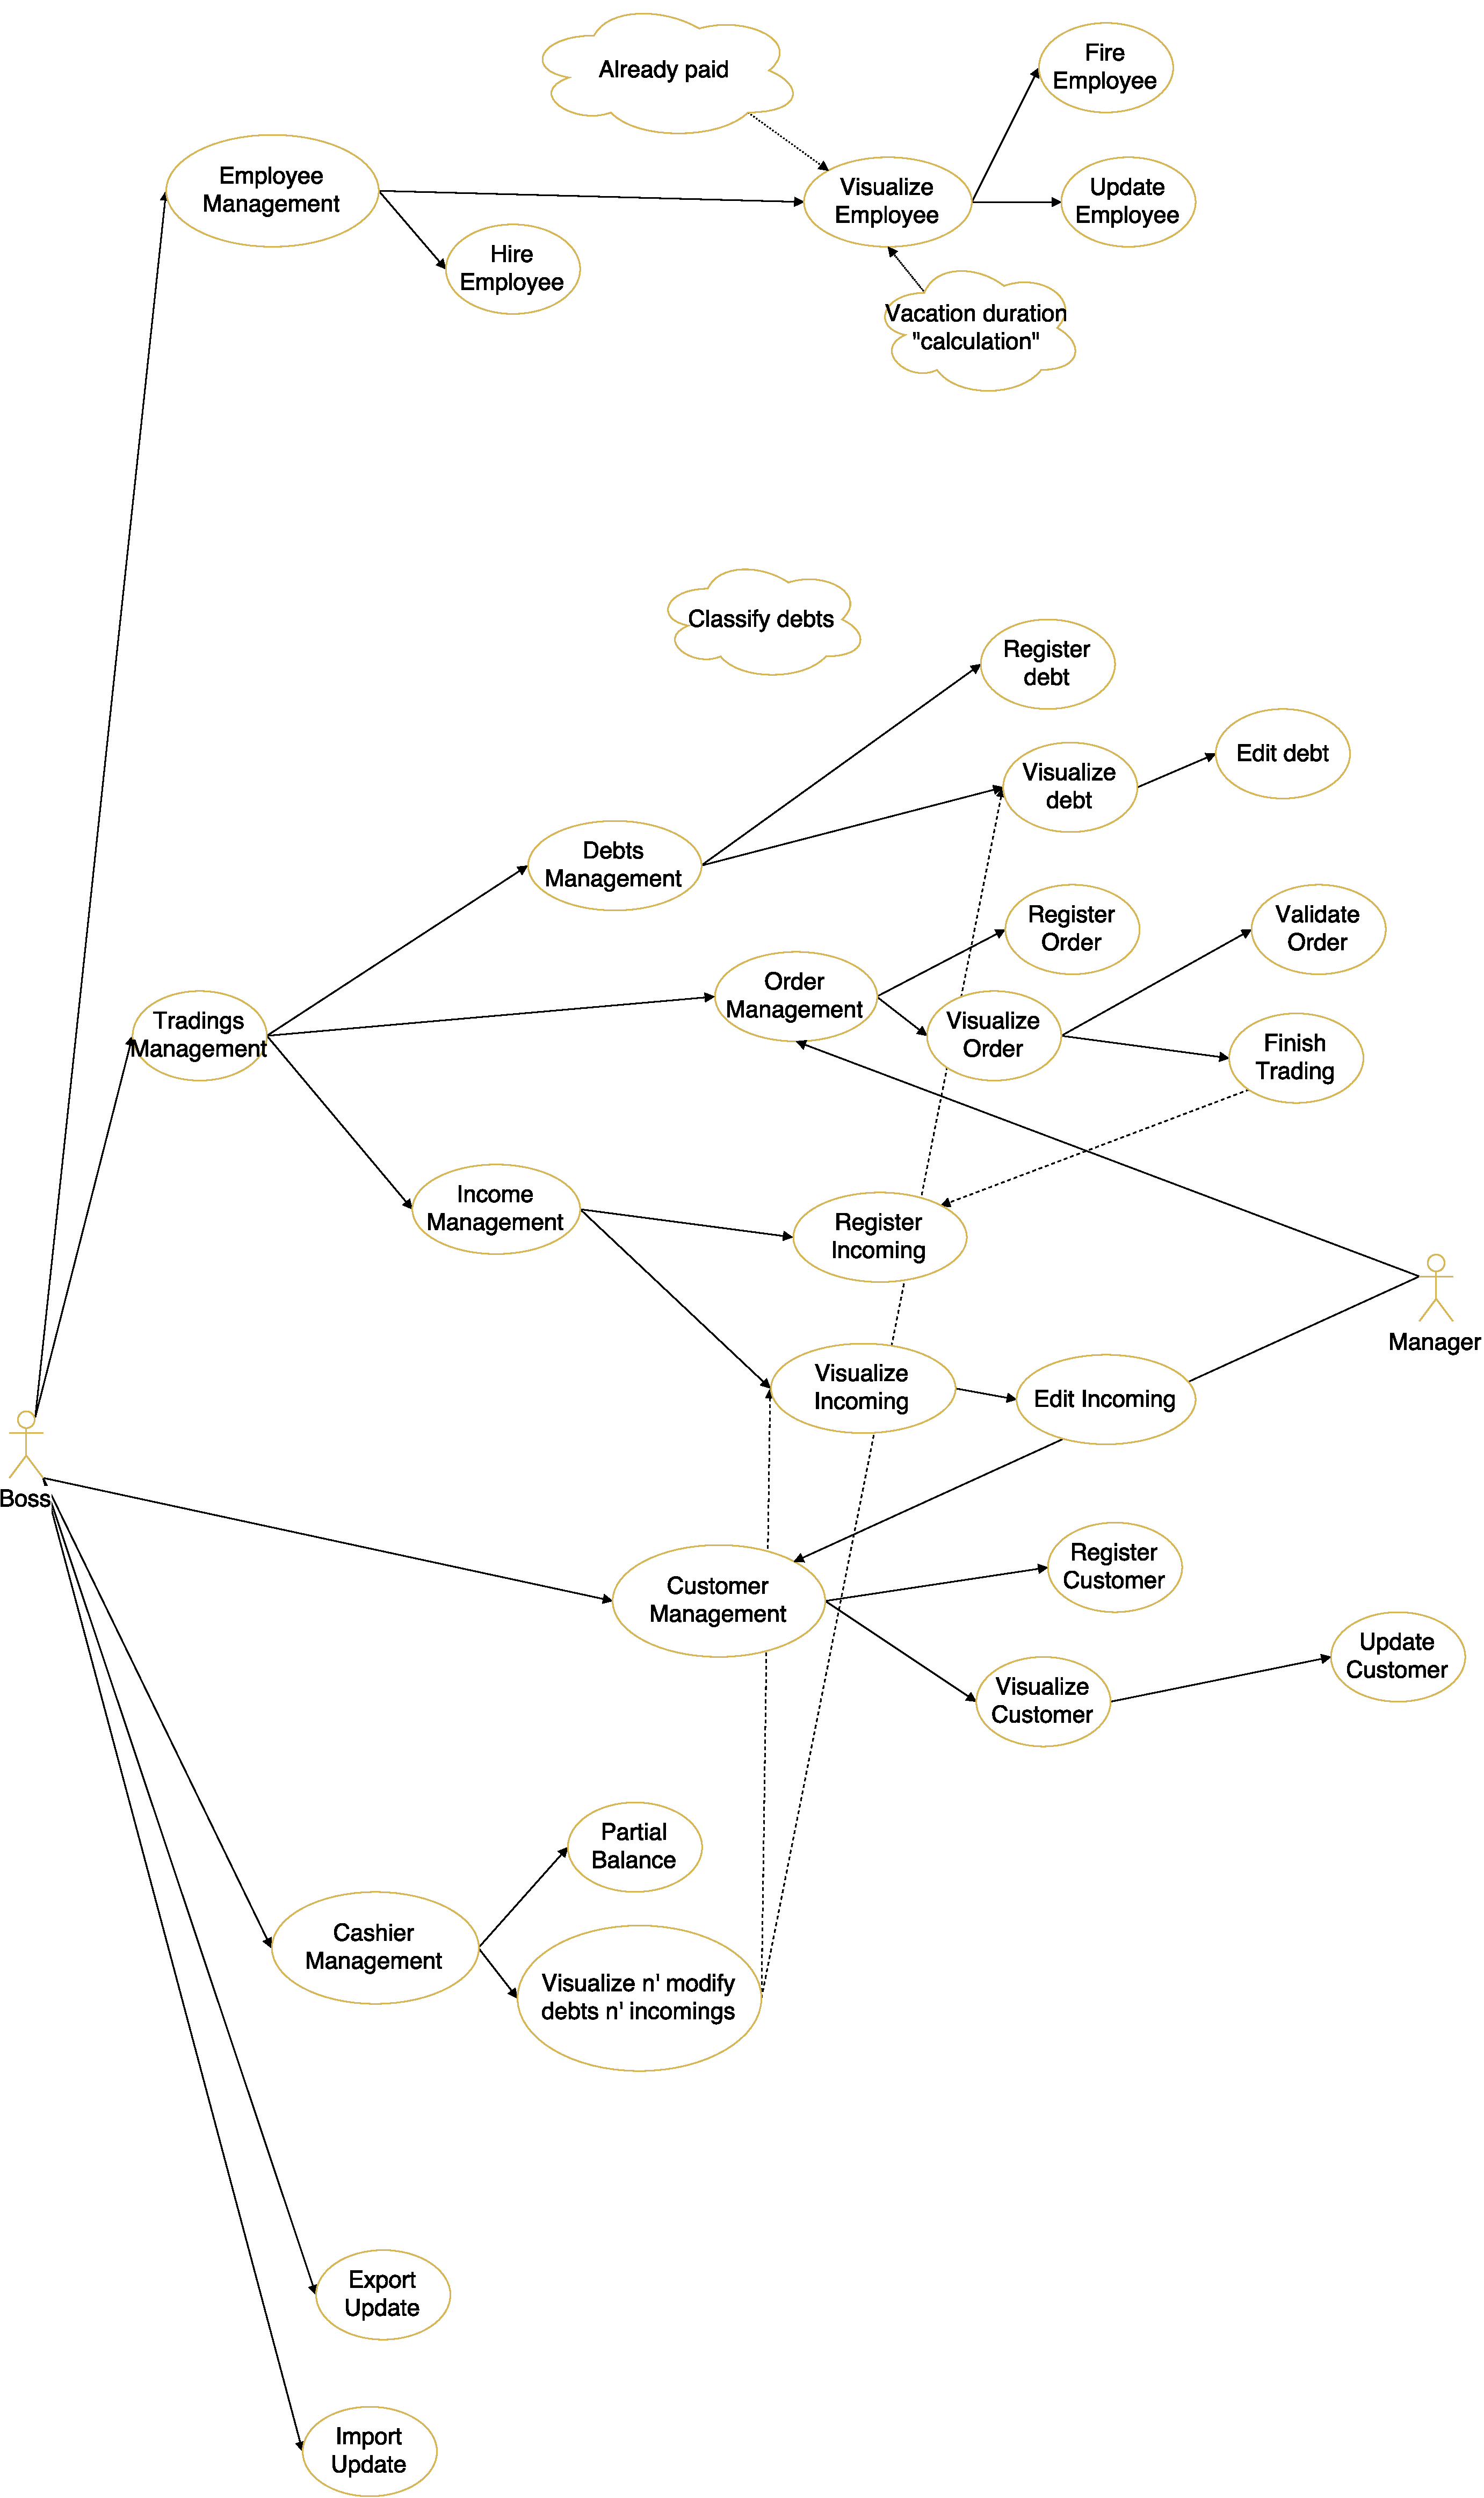
\includegraphics[width=\textwidth]{./UseCasesDiagramEnglish.pdf}
		\end{figure}
		\begin{figure}[H]
			\centering 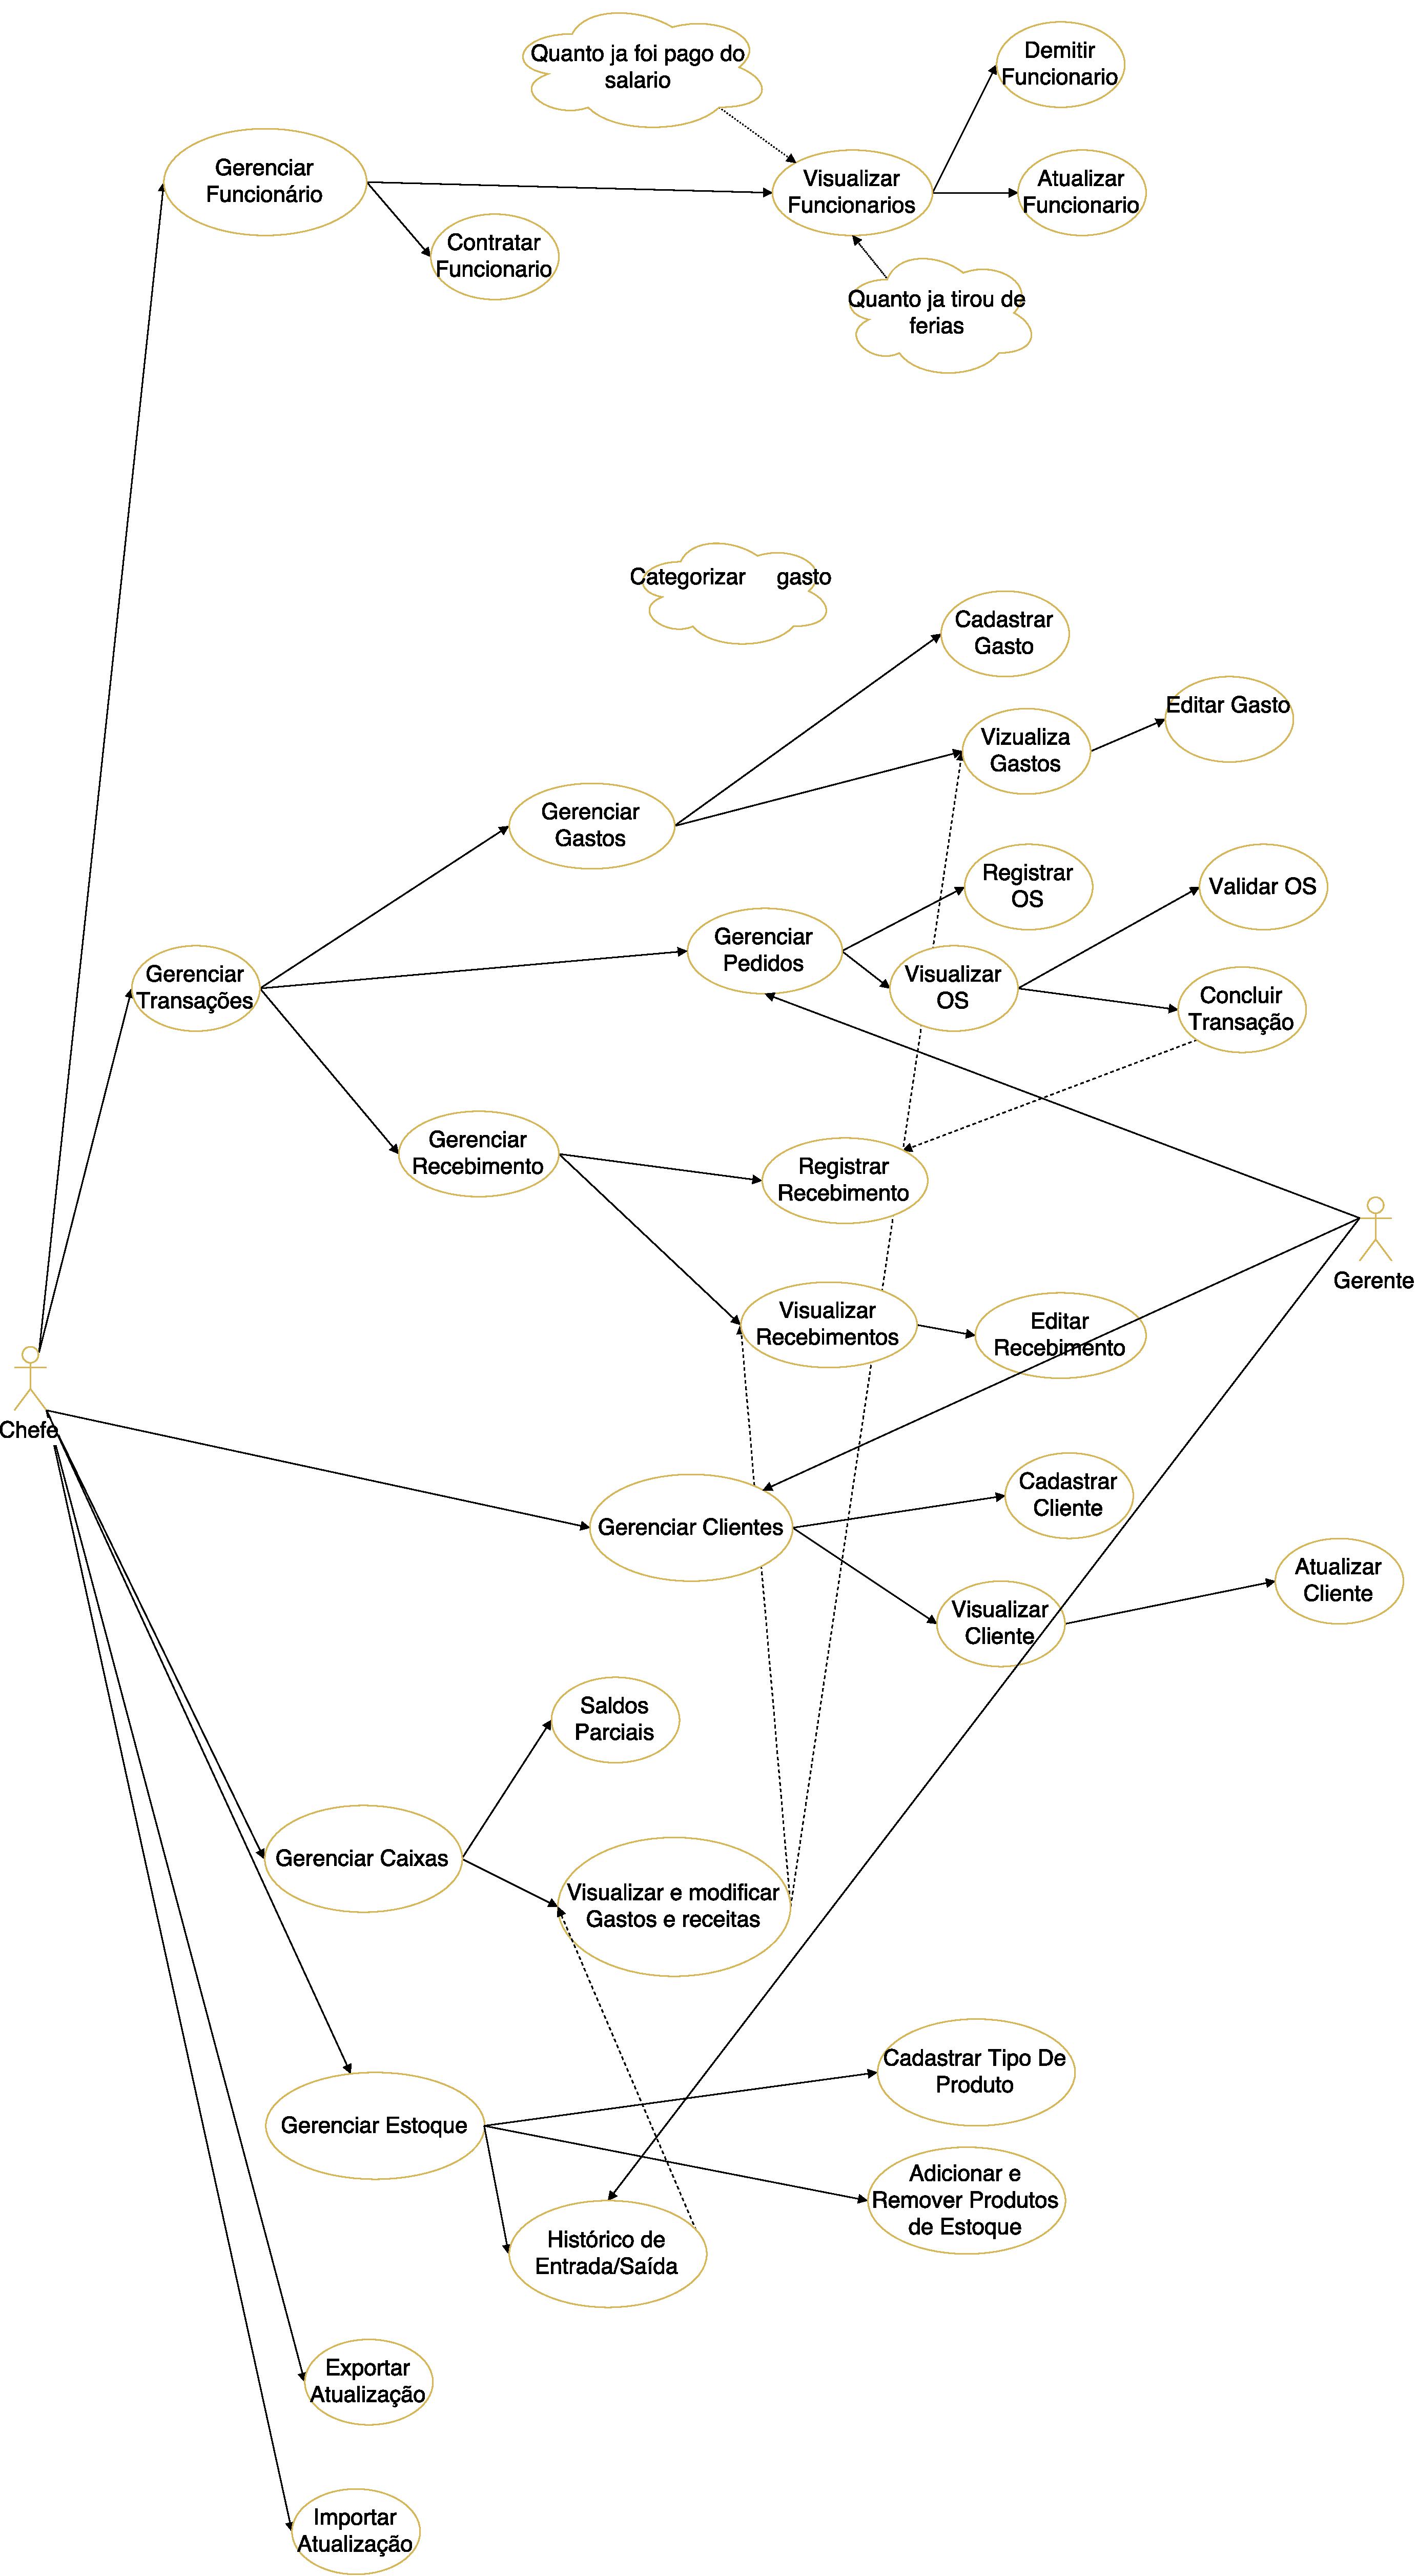
\includegraphics[width=\textwidth]{./DiagramaCasoDeUsoOficinaOld.pdf} 
		\end{figure}
		\begin{figure}[H]
			\centering 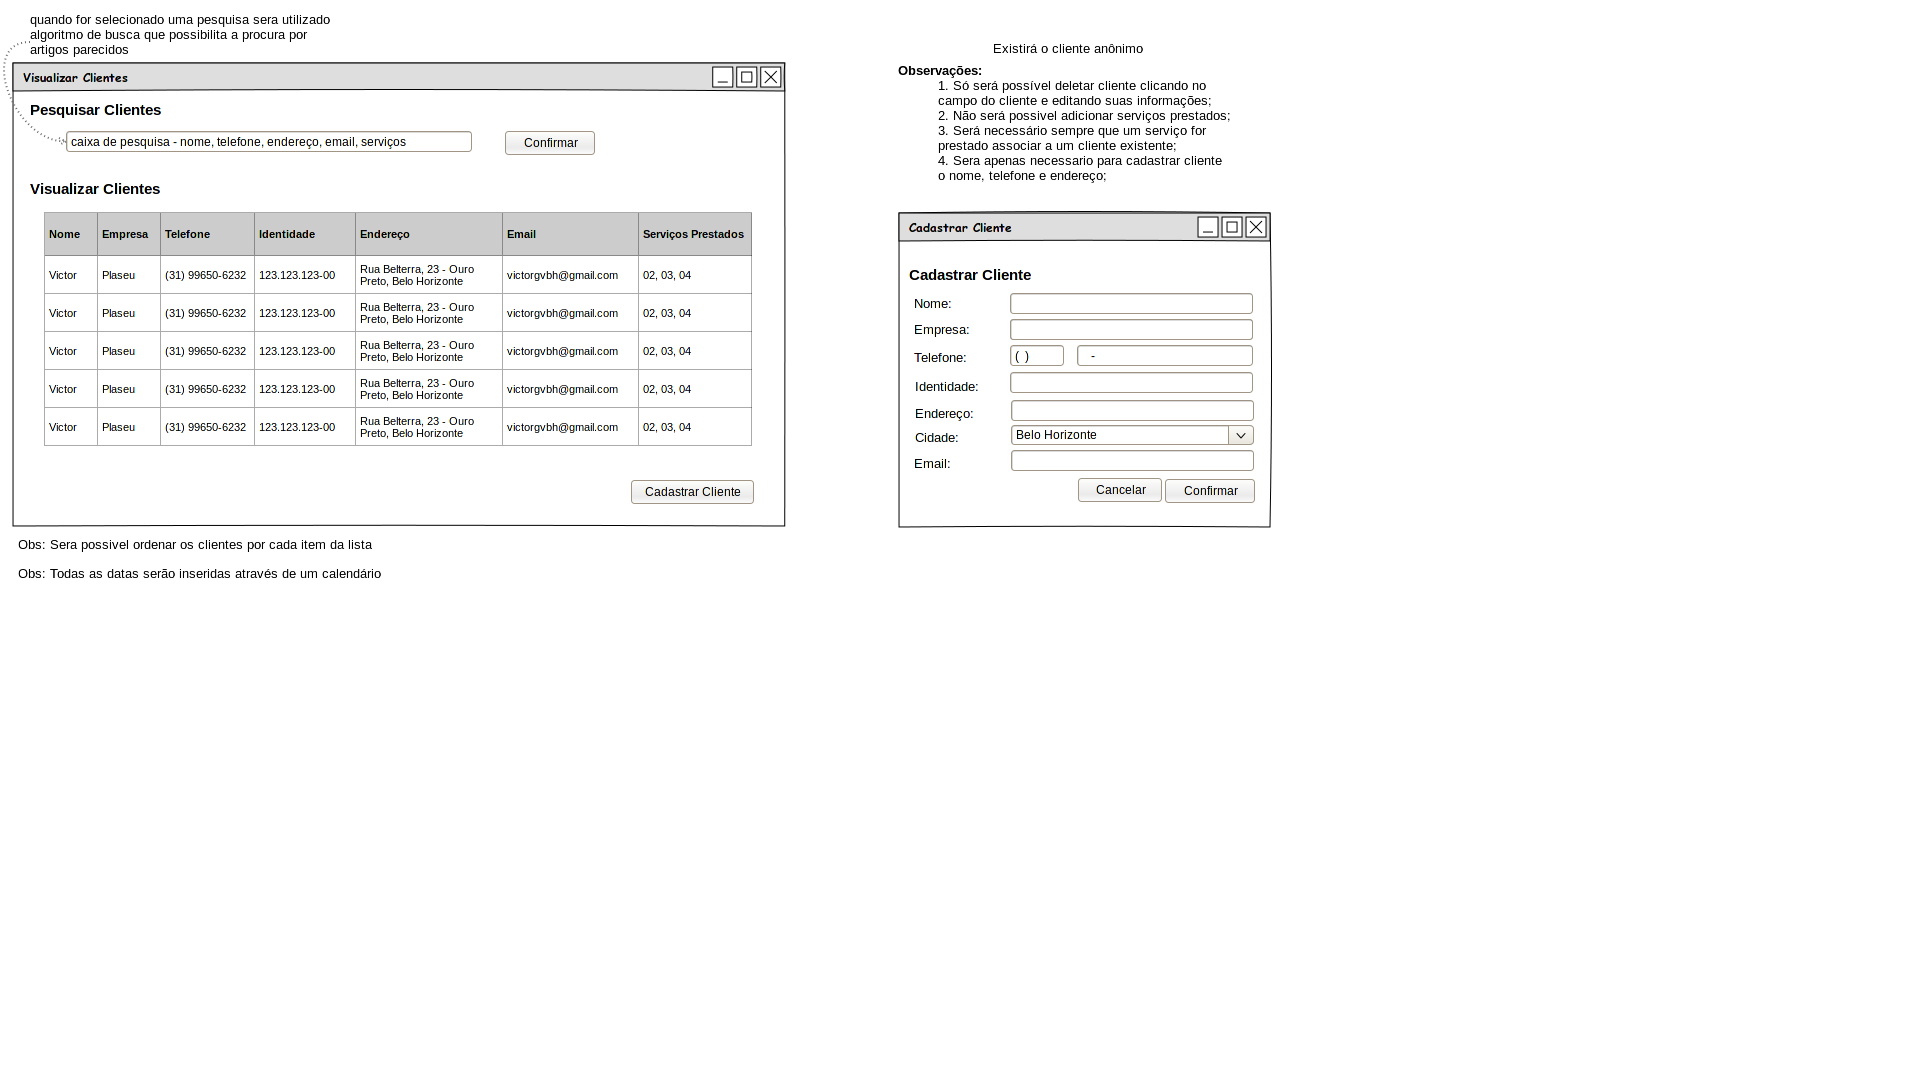
\includegraphics[width=\textwidth]{./Gerenciar Cliente.png}
		\end{figure}
		\begin{figure}[H]
			\centering 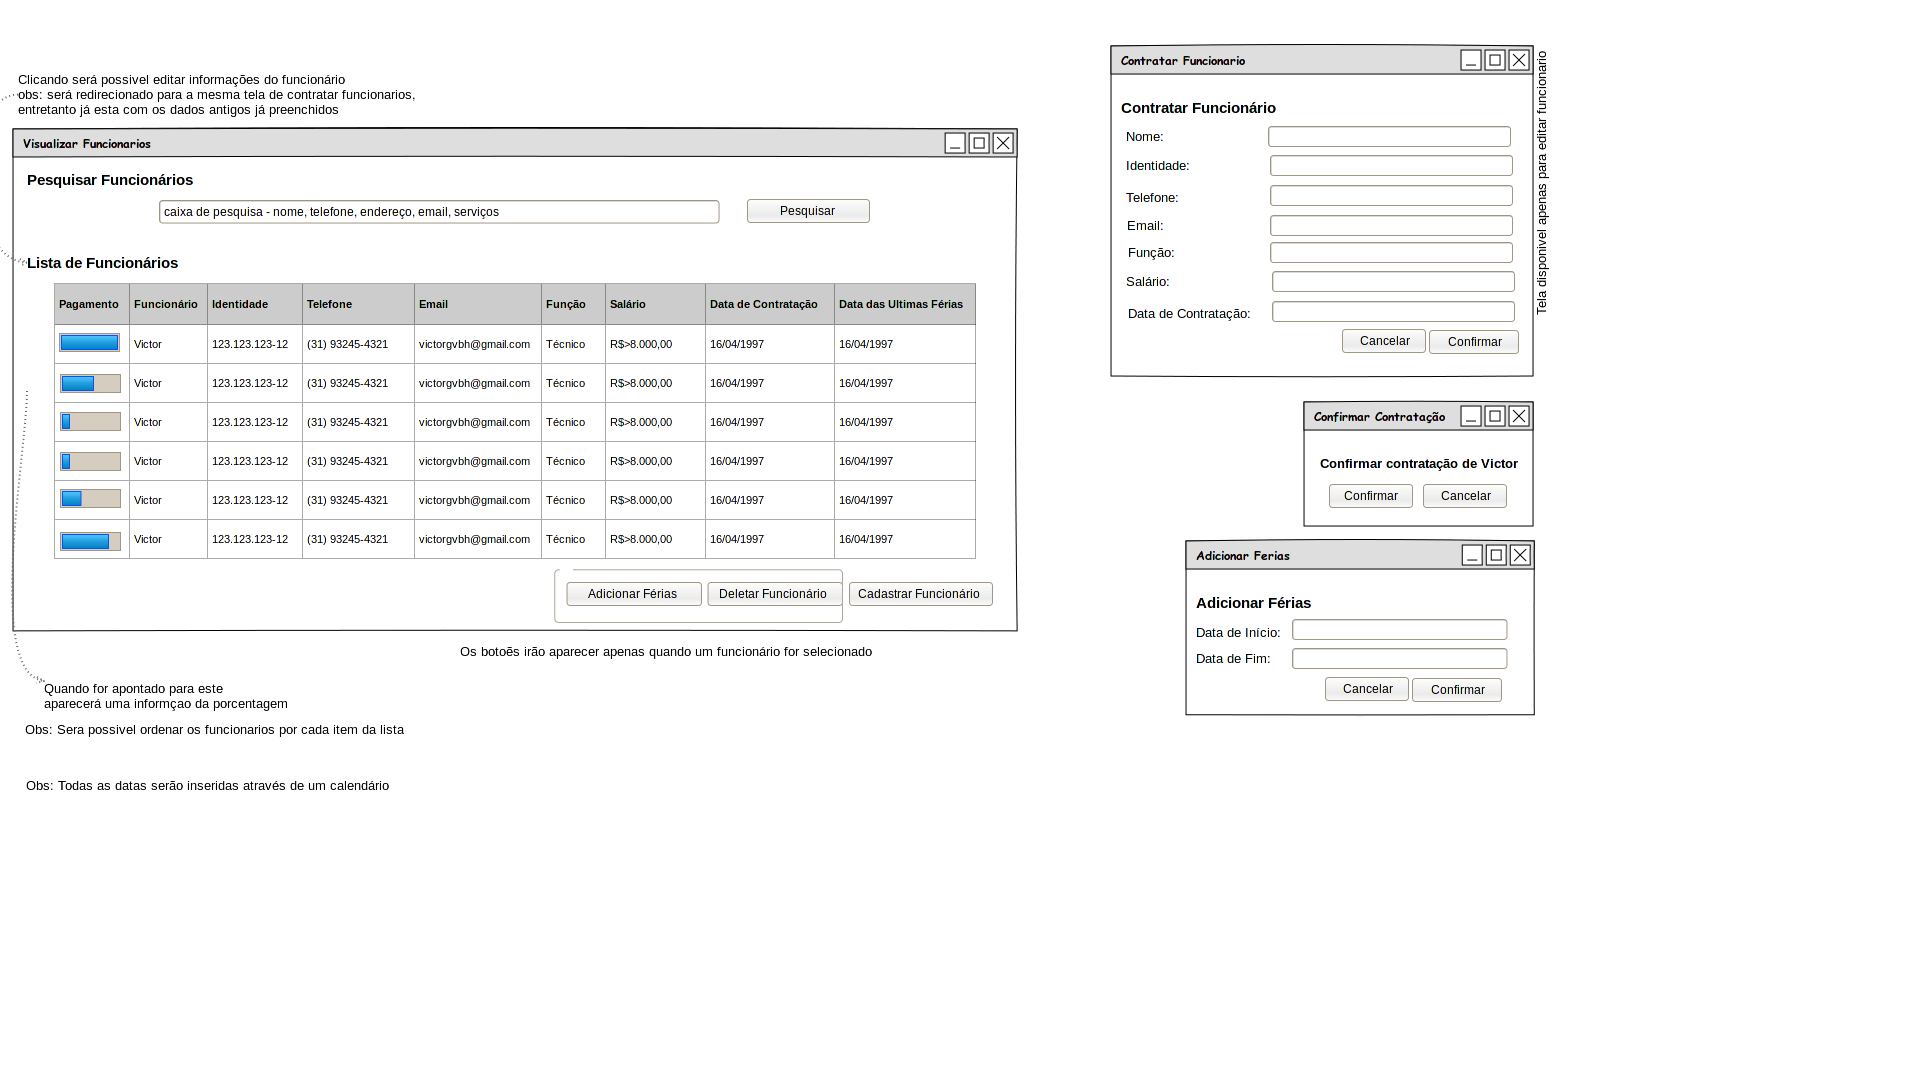
\includegraphics[width=\textwidth]{./Gerenciar Funcionario.png} 
		\end{figure}
		\begin{figure}[H]
			\centering 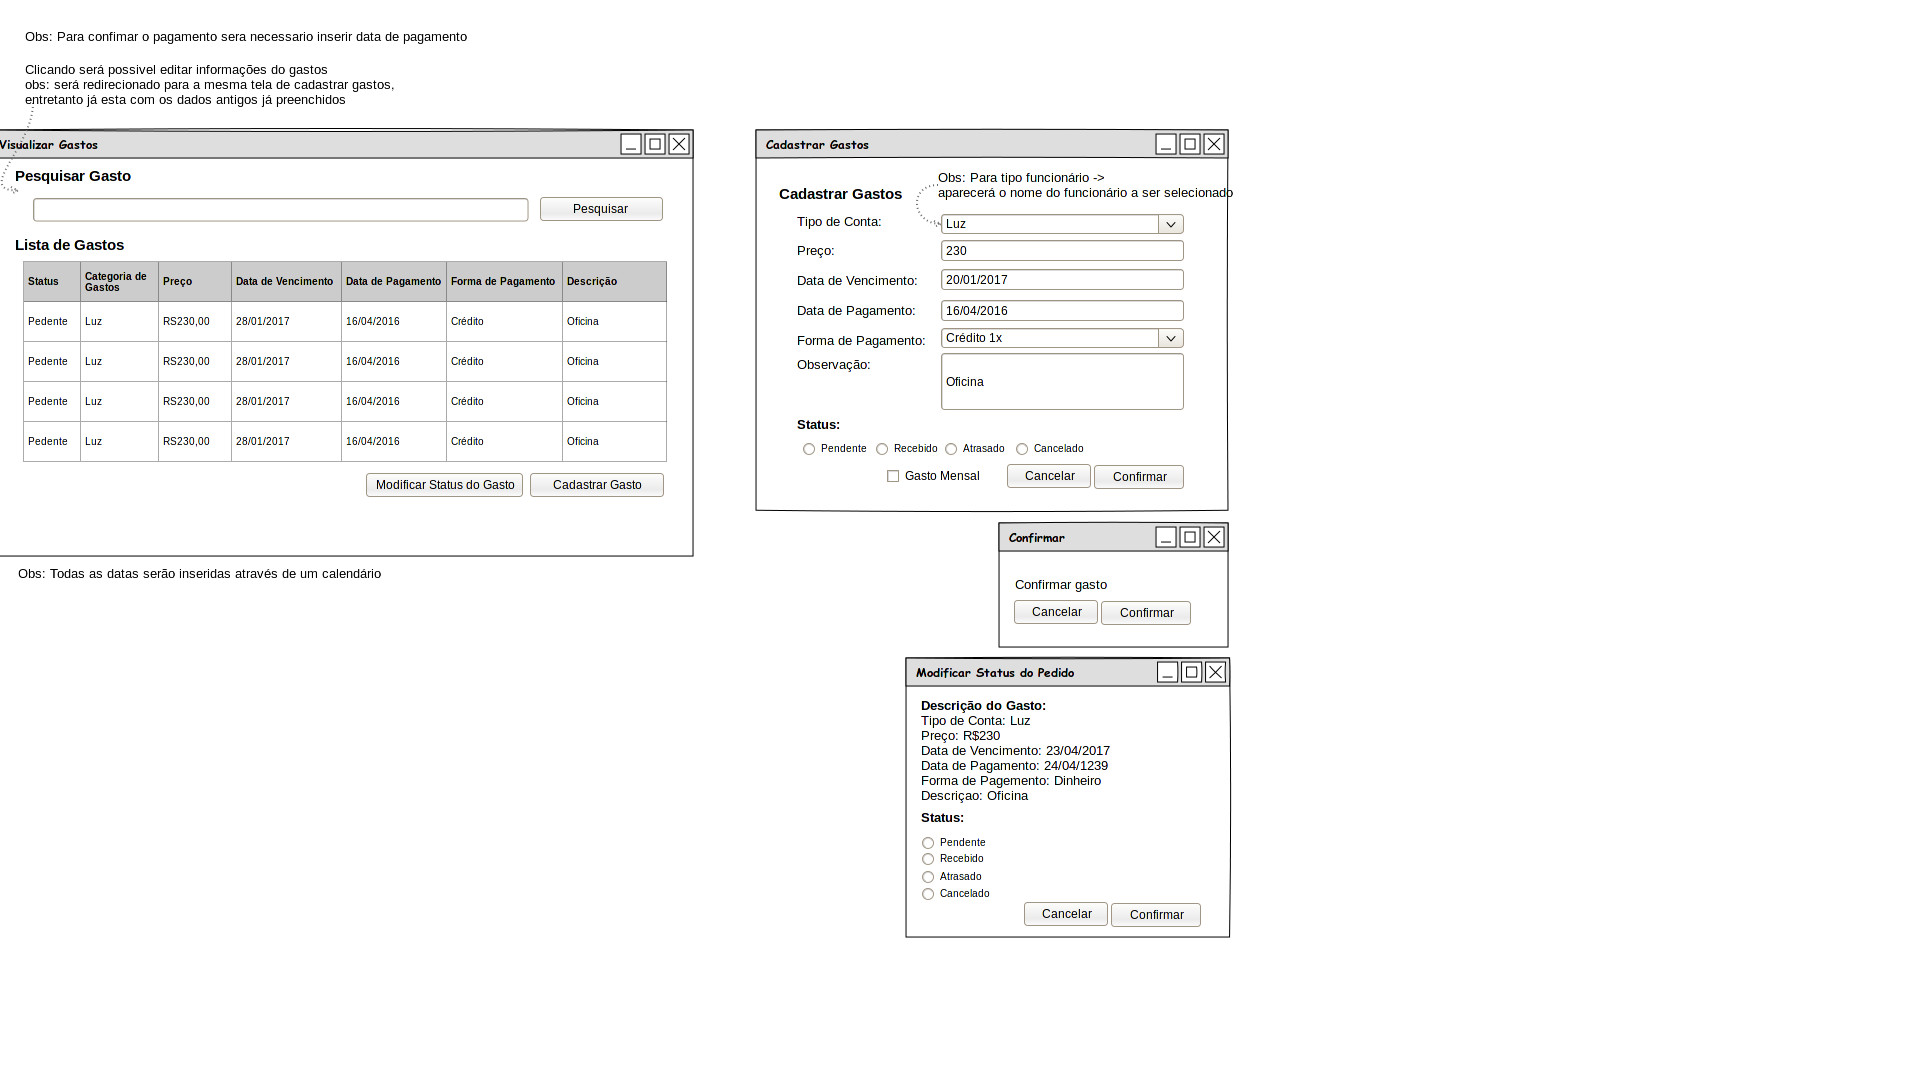
\includegraphics[width=\textwidth]{./Gerenciar Gastos.png} 
		\end{figure}
		\begin{figure}[H]
			\centering 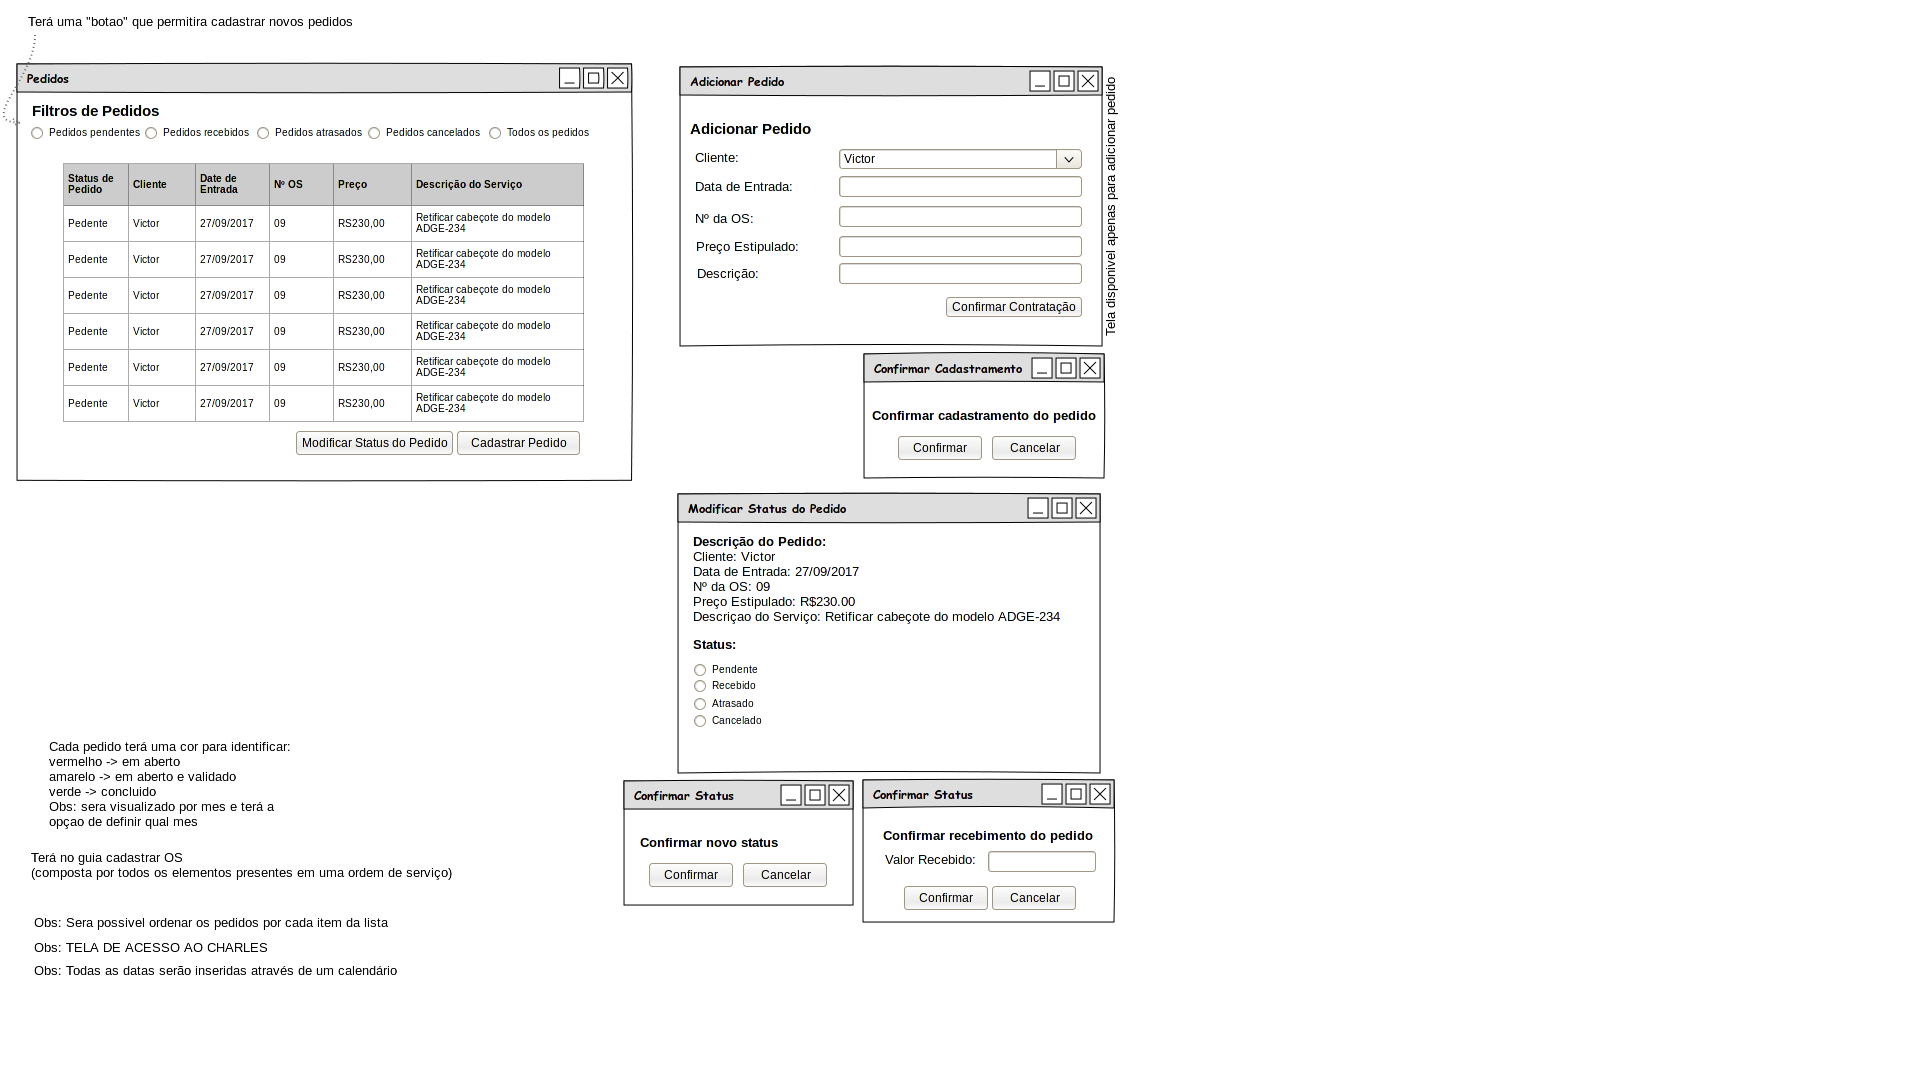
\includegraphics[width=\textwidth]{./Gerenciar Pedidos.png}
		\end{figure}
		\subsection{Licença} 
		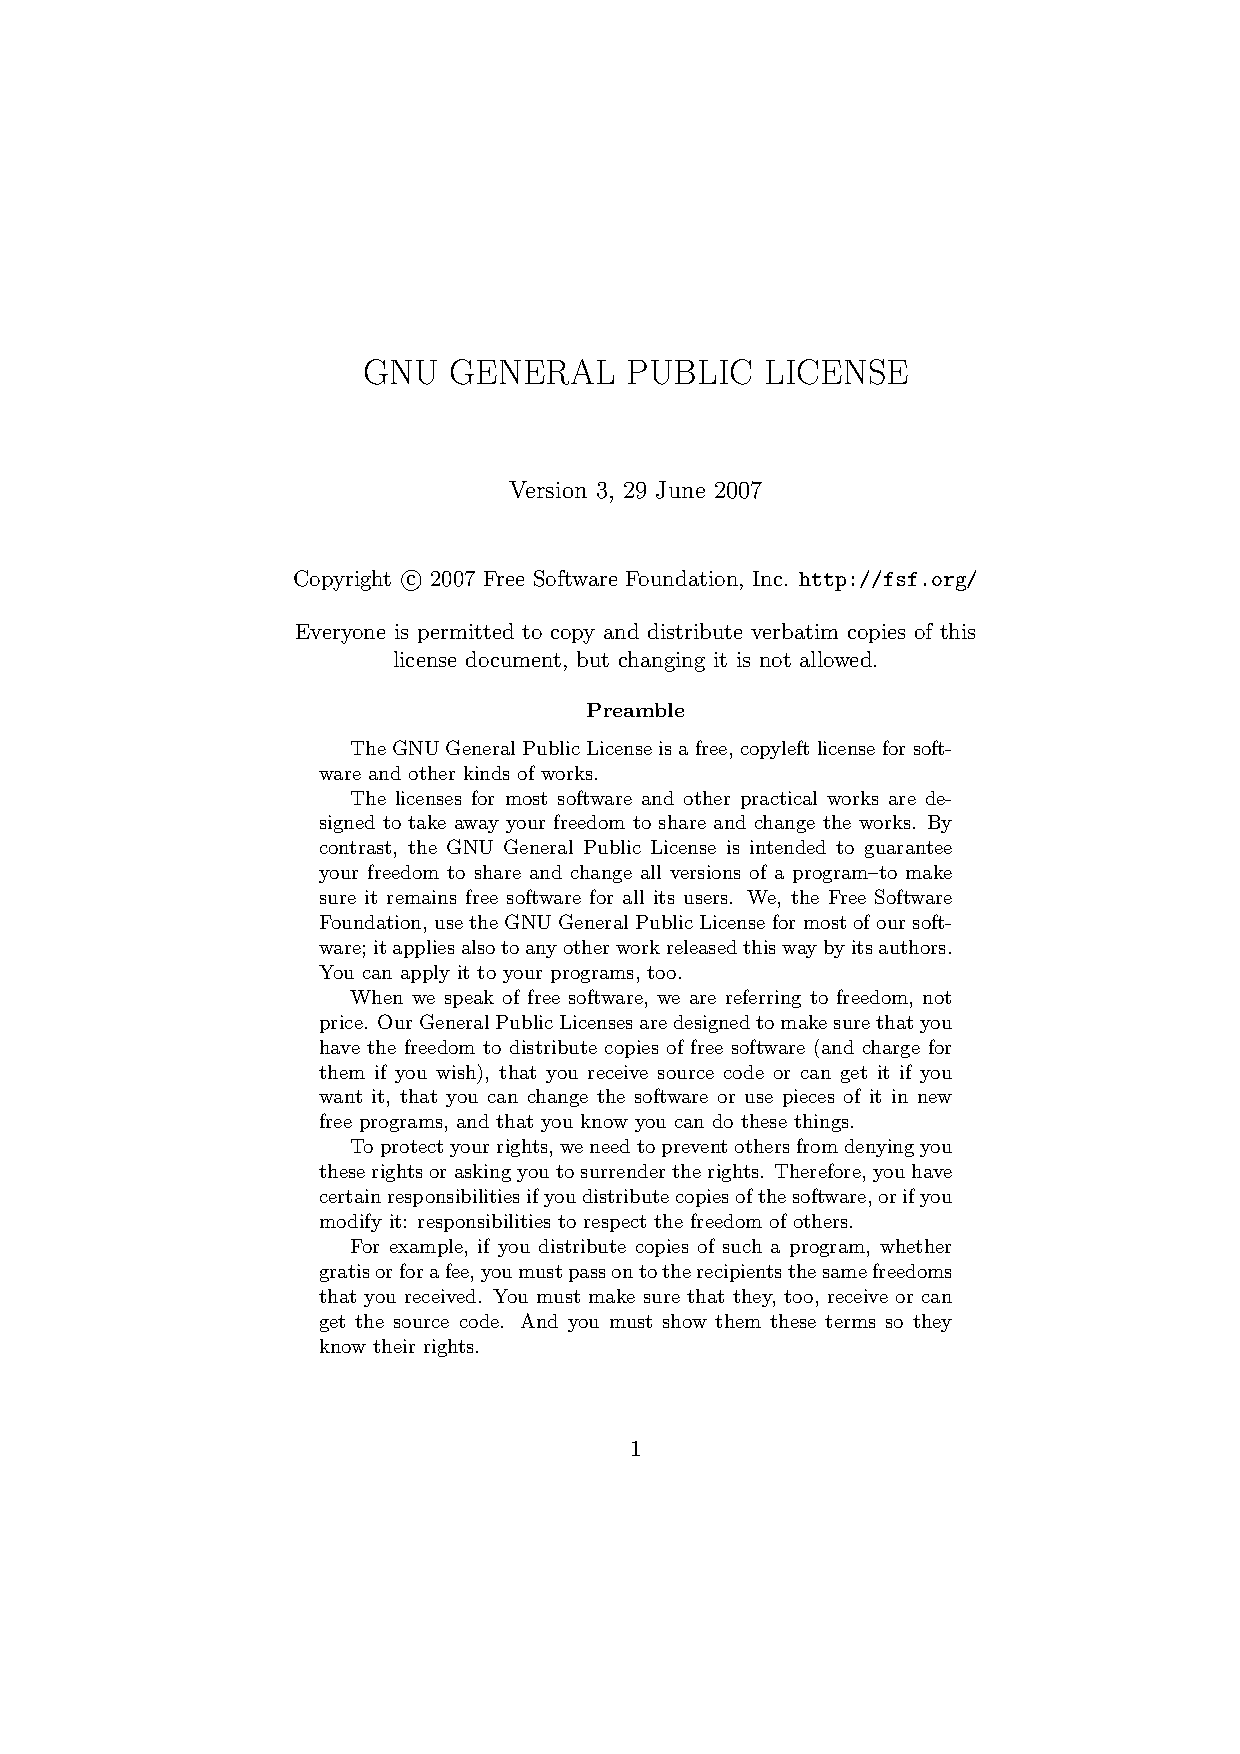
\includepdf[pages=-]{./gpl-3-0.pdf}
		\subsection{Códigos Fontes incorporados ao programa}
		
		Por Enquanto Nenhum...
		%TODO Completar as seguintes seções
		
%	\section{Tutoriais e FAQ}
%		\subsection{Como contribuir para o projeto?}
%		\subsection{Qual expectativa da data de conclusão?}
%		\subsection{Como instalar esse software?}
%		\subsection{Como utilizar esse software?}
%		\subsection{Como adotar esse software em minha empresa? Existe algum tipo de suporte?}
%		\subsection{Já baixei e utilizei, mas encontrei problemas ou coisas que poderiam ser adicionadas. Como entro em contato?}
%		\subsection{Qual a vantagem de utilizar esse software?}
%		\subsection{Por que C++, gtkmm e SQLite?}
%	\section{Referência}
%	\section{Agradecimentos}
\end{document}
